%%indent: 
%chapt: 0
%  sec: 2
%    subsec:4
%      subsubsec:6
%  text: previous+2


\chapter{\texorpdfstring{DU$\nu$E}{DUNE} une expérience d'oscillation de neutrinos d'accélérateur à longue ligne de base de troisième génération}
\chapterprecishere{
``Potentielle citation sans aucun rapport avec le sujet"\par\raggedleft--- \textup{Personne inconnue}, contexte à déterminer
}

  Nous avons vu au chapitre précédent que la découverte des oscillations des neutrinos à la fin des années 90 a montré que les neutrinos peuvent changer de saveur durant leur propagation, impliquant que les neutrinos ont une masse. La matrice \gls{pmns} décrivant ces changements de saveur a été étudiée depuis par différents types d'expériences afin de mesurer avec précision ses 4 paramètres (3 angles de mélange et une phase de violation de CP), dont dépendent les amplitudes d'oscillation des probabilités de changement de saveur, ainsi que les différences de masse au carré des neutrinos, dont dépendent les fréquences de ces oscillations. Les deux principales questions encore non résolues dans le domaine des oscillations des neutrinos sont l'ordre des masses de ces derniers, qui contraint plusieurs modèles au delà du modèle standard, ainsi que la valeur de la phase de violation de CP. Une valeur différente de 0 et $\pi$ pourrait expliquer l'asymétrie matière-antimatière visible dans l'univers.

  \begin{figure}[htbp]
    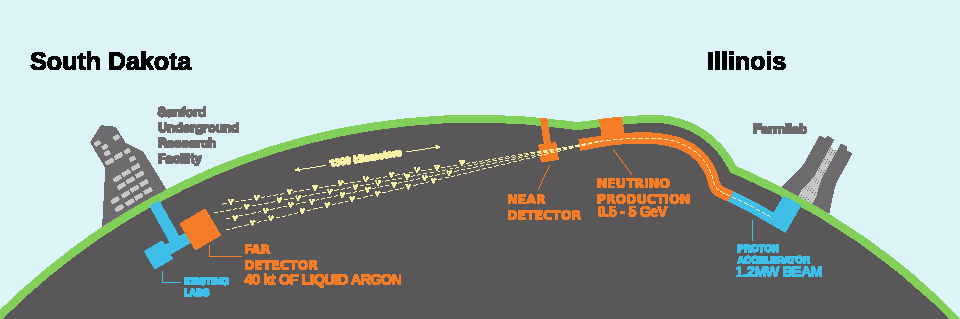
\includegraphics[width=\textwidth]{dune.pdf}
    \caption[L'expérience \acrshort{dune}]{\label{fig::dune}L'expérience \acrshort{dune} au États-Unis enverra à partir de 2026 un faisceau de neutrinos muoniques vers le site de Sanford, à \SI{1300}{\kilo\meter}, afin d'étudier la violation de CP dans le secteur leptonique et l'ordre des masses des neutrinos.}
  \end{figure}

  L'expérience \gls{dune} (voir \autoref{fig::dune}) vise à déterminer l'ordre des masses et à vérifier si la symétrie de CP est brisée dans le secteur des neutrinos. Pour ce faire, \gls{dune} mesurera la probabilité de transition $P\left(\nuanu_{\mu}\to\nuanu_e\right)$ et la probabilité de survie $P\left(\nuanu_{\mu}\to\nuanu_{\mu}\right)$ de (anti)neutrinos d'accélérateur, produits au Fermilab (illinois) et détectés à Sanford (Dakota du sud). Sa longue ligne de base de \SI{1300}{\kilo\meter} permettra de profiter des effets de matières, sensibles à l'ordre des masses. Les énergies des neutrinos du faisceau seront comprises entre \SI{0.5}{\giga\electronvolt} et \SI{5}{\giga\electronvolt}, afin de couvrir deux maxima de probabilité de transition, permettant de discerner les effets de matière des effets dues à la possible violation de CP. Le projet a vu le jour suite à l'annonce par le ministère de l'énergie des États-Unis de sa volonté d'améliorer le dispositif de faisceau du Fermilab avec la mise à niveau PIP-2, permettant de disposer d'un faisceau de $\SI{1.2}{\mega\watt}$. Le premier rapport d'étude conceptuel de \gls{dune} de 4 volumes a été publié en 2016. Le projet regroupe aujourd'hui un millier de collaborateurs, répartis dans 175 institutions et 32 pays.

  Les constructions civiles du détecteur lointain, à l'installation de recherche souterraine de Sanford, ont commencé en 2017 avec le début des excavations. Elles seront suivies par les installations cryogéniques, nécessaires aux opérations utilisant de l'argon liquide, qui est le composant principal du détecteur. Ce dernier sera composé de 4 modules de \gls{lartpc} pour un total de \SI{40}{\kilo\tonne}. Ces modules seront progressivement installés, la mise en service et les premières prises de données du premier module étant prévues pour 2024\cite{Acciarri2016}. Le dernier module devrait commencer à prendre des données vers 2028. Une variante de la technologie \gls{lartpc} est en cours d'étude par le projet  \gls{wa105}proto\gls{dune}-DP, dont les prototypes, au \gls{cern}, sont l'objets de cette thèse. Cette variante permet d'amplification des charges dans une fine couche d'argon gazeux, d'où son nom de \gls{dlartpc}. En parallèle, l'injecteur principale NuMI du Fermilab, qui a fourni les neutrinos des expériences \gls{nova} et \gls{minos}, sera mis à niveau par le projet PIP-II qui permettra d'atteindre une puissance de \SI{1.2}{\mega\watt} d'ici 2026, ce qui en fera le faisceau de neutrinos le plus intense de la planète. Une autre mise à niveau, PIP-III, est prévue pour 2030 et permettra d'atteindre \SI{2.4}{\mega\watt}.

  La première section de ce chapitre présente un résumé des expériences d'oscillation des neutrinos d'accélérateur à longue ligne de base, passées, actuelles et futures. La seconde section est dédiée à \gls{dune}, où y sont présentés ses objectifs et les sensibilités attendues. La troisième section décrira le fonctionnement de son faisceau de neutrino, de son détecteur proche et de son détecteur lointain et présentera leur performances requises et attendues.

  \section{Les expériences d'oscillation de neutrinos d'accélérateurs à longue ligne de base}

%    %Généralités sur DUNE: où, quand, pourquoi.
%    \gls{dune} est une expérience d'oscillation des neutrinos à longue ligne de base, qui enverra un faisceau de neutrino depuis le Fermilab (Illinois) vers l'installation de recherche souterraine de Sanford (Dakota du sud)(voir \autoref{fig::dune}). Comme toutes les expériences de neutrinos d'accélérateur à longue ligne de base, ses constituants essentiels sont un faisceau de neutrino, un détecteur proche servant à caractériser ce faisceau avant changement de saveurs, et un détecteur lointain servant à effectuer les mesures après changement de saveur.
%    
%    Le faisceau de neutrinos, détaillé en \autoref{sec::faisceau}, sera créé au Fermilab. Après avoir parcouru \SI{300}{\meter}, il traversera un détecteur proche où ses différentes caractéristiques (flux, composition, énergies...) seront mesurés afin de réduire au maximum les incertitudes systématiques puis parcourra une ligne de base de \SI{1300}{\kilo\meter} à travers la croûte terrestre avant d'atteindre le détecteur lointain à Sanford, à \SI{1475}{\meter} de profondeur. C'est dans ce détecteur que s'effectuera la plus grande partie des mesures de physique. Il sera composé de quatre modules de \glspl{tpc} chacune remplie d'argon liquide pour un total de $\SI{40}{\kilo\tonne}$. Les détails de cette technologie sont discutés en \autoref{sec::lartpc}.
%    
%    Comme nous l'avons vu en \autoref{sec::oscillations}, les probabilités de changement de saveur oscillent en fonction de $L/E$, où $L$ est la distance parcourue par les neutrinos (ligne de base) et $E$ leur énergie. Il est possible d'optimiser le ratio $L/E$ afin d'observer des neutrinos à un maximum de probabilité de changement de saveur. En plus de cela, l'expérience \gls{dune} cherche à se placer à une ligne de base suffisamment importante pour que les effets de matière permettent la mesure de l'ordre des masses grâce à l'effet de résonance \gls{msw}. La ligne de base choisie, de \SI{1300}{\kilo\meter}, doit être accompagnée d'une énergie autour de \SI{2.5}{\giga\electronvolt} (voir \autoref{fig::3flavors_oscillations}) afin d'atteindre le premier maximum de probabilité. Il est également possible, en générant un faisceau de neutrino à large spectre, de couvrir le second maximum, où les effets due à $\delta_{CP}$ sont plus importants. Ce maximum est situé autour de \SI{0.9}{\giga\electronvolt}. Les neutrinos du faisceau que détectera \gls{dune} auront une énergie comprise entre \numprint{0.5} et \SI{5}{\giga\electronvolt}, couvrant ainsi les deux maxima.

    \subsection{Qu'est ce qu'une expérience d'oscillation de neutrinos d'accélérateurs à longue ligne de base?}

      Les expériences d'oscillation de neutrinos d'accélérateurs à longue ligne de base cherchent à mesurer les probabilités de transition $P\left(\nuanu_{\mu}\to \nuanu_e\right)$ et de survie $P\left(\nuanu_{\mu}\to \nuanu_{\mu}\right)$ en fonction de l'énergie du (anti)neutrino incident en détectant les produits de réaction des neutrinos d'un faisceau initialement composé uniquement de (anti)neutrinos muoniques. Ce faisant, ces expériences ont accès aux angles de mélanges des secteurs atmosphériques et réacteurs de la matrice \gls{pmns} décrits en \autoref{sec::current_knowledge}, ainsi qu'à la phase de violation de CP et au signe des différences de masse au carré dont dépendent notamment les effets de matière via la résonance MSW décrite en \autoref{sec::matter_effect}. Si ces effets, qui augmentent avec la ligne de base, sont suffisamment importants, ces expériences peuvent sonder l'ordre des masses des neutrinos.
    
      Le système de détection d'une telle expérience doit donc être capable de différencier efficacement le signal recherché (les réactions de neutrino muonique et de neutrino électronique par courant chargé) des différents bruits de fond, ce qui nécessite une bonne résolution spatiale, ainsi que de mesurer précisément l'énergie mise en jeu dans ces réactions afin d'observer l'allure des probabilité de changement de saveur en fonction de $E$. Le faisceau de neutrino, dont le principe est décrit en \autoref{sec::faisceau}, va d'abord traverser un détecteur placé proche de la source, typiquement à quelques centaines de mètres, quand la probabilité d'oscillation est encore nulle. Les caractéristiques importantes du faisceau y sont analysées, comme le flux et le spectre en énergie, afin de contraindre au maximum les différents paramètres et de réduire les erreurs systématiques. Le faisceau parcours ensuite une grande distance à travers la croûte terrestre jusqu'au détecteur lointain. 
    
      La possibilité de comparer les observations avant et après propagation d'une même source de neutrinos est une plus-value des expériences à longue ligne de base utilisant des faisceaux ou des réacteurs. Une plus-value du faisceau est son ajustabilité en flux et en énergie. Le spectre en énergie peut être choisie précisément, dans une gamme d'énergie allant de \SI{0.5}{\giga\electronvolt} à \SI{100}{\giga\electronvolt}. Il est possible de choisir une gamme d'énergie très restreinte en plaçant le détecteur légèrement en dehors de l'axe, ou au contraire de couvrir une gamme d'énergie plus grande en se plaçant en face. De plus, il est possible de choisir entre un faisceau de neutrino ou d'antineutrino. Bien que la mesure de l'oscillation des neutrinos seule suffise théoriquement à mesurer la phase de violation de CP et l'ordre des masses (voir \autoref{sec::3flavor_matter}), la comparaison à l'oscillation d'anti-neutrino permet de gagner en précision, et de mettre directement en évidence l'asymétrie matière-antimatière dans le secteur leptonique. 

    \subsection{Expériences passées, actuelles et futures}

      Les expériences à longues ligne de base avec neutrinos d'accélérateurs sont apparues dans la fin des années 90. Les premières et deuxièmes générations ont confirmé les observations indiquant l'existence des oscillations des neutrinos, et ont effectué des mesures de précisions sur les angles $\theta_{13}$ et $\theta_{23}$ ainsi que sur la différence de masse au carré $\Delta m^2_{32}$\cite{pdg2018}. Les expériences de première génération étaient, dans l'ordre chronologique, \gls{k2k}\cite{Collaboration2006a} (Japon, 1999--2004), \gls{minos}\cite{Collaboration2014} (USA, 2005-2011), \gls{opera}\cite{Agafonova2018} (Europe, 2008--2012) et \gls{icarus} (Europe, 2004--2013). La seconde génération, encore en activité, sont les expériences \gls{nova}\cite{Adamson2016} (USA, 2014--) et \gls{t2k}\cite{Abe2018} (Japon, 2010--). Les expériences de la troisième génération, en développement, sont \gls{t2hk}\cite{HK2018} dont le début des travaux est prévue au Japon pour  2020 et \gls{dune}\cite{Acciarri2016}, prévue aux USA pour 2026. Ces dernières ont pour but la détermination de la violation de CP, dont une valeur de $\delta_{CP}$ différente de $0$ et $\pi$ a été annoncée avec un niveau de confiance de $2\;\sigma$ par \gls{t2k}\cite{Abe2018} en 2011, et l'ordre des masses.

      \subsubsection{Les expériences de première génération}

        \paragraph{\gls{k2k}\cite{Collaboration2006a}:} C'était la première expérience de faisceau à longue ligne de base, construite dans le but de vérifier les résultats de Super-Kamiokande sur les oscillations des neutrinos atmosphériques. Un faisceau de neutrinos muoniques produit par un synchrotron de proton de $\SI{12}{\giga\electronvolt}$ au KEK, Tsukuba, Japon, parcourait $\SI{300}{\meter}$ jusqu'à un détecteur proche Cherenkov à eau de $\SI{1}{\kilo\tonne}$. Le faisceau traversait ensuite $\SI{250}{\kilo\meter}$ jusqu'à Super-Kamiokande, un détecteur Cherenkov à eau de $\SI{50}{\kilo\tonne}$. \gls{k2k} a permit de montrer à un niveau de confiance de $4.3\;\sigma$ que les neutrinos muonique disparaissait, apportant ainsi une confirmation de la théorie des oscillations des neutrinos. \gls{k2k} a également fournit une mesure de la différence des masses carrées de $|\Delta m^2_{32}|=2.8^{+0.7}_{-0.9}\times\SI{e-3}{\electronvolt\squared}$.

        \paragraph{\gls{minos}\cite{Collaboration2014}:} L'expérience \gls{minos} avait pour but de mesurer avec une plus grande précision le secteur atmosphérique. Elle observait la disparition des neutrinos muoniques de $\SI{3}{\giga\electronvolt}$ produits par la ligne de faisceau NuMi, au fermilab, avec une ligne de base de \SI{735}{\kilo\meter}. Le détecteur lointain, un calorimètre à échantillonnage en acier scintillateur de $\SI{5.4}{\kilo\tonne}$, était situé dans le Minnesota du nord. Elle a mesuré la différences de masse au carré $\Delta m_{32}^2 = 2.35^{+0.11}_{-0.08}\times\SI{e-3}{\electronvolt\squared\per c^4}$ et l'angle $\sin^2(2\theta_{23}) > 0.91$ (limite de confiance de 90\,\%). 

        \paragraph{\gls{opera}\cite{Agafonova2018}:} L'expérience \gls{opera} diffère légèrement des autres expériences à longue ligne de base d'accélérateur par le fait qu'elle cherchait à observer l'apparition de neutrino tauique, et non l'apparition de neutrinos électroniques ou la disparition de neutrinos muoniques. Elle faisait parti du programme \gls{cngs} dont le but était l'étude de l'hypothèse des oscillations des neutrinos. Elle utilisait un trajectographe à émulsion, constitué de \numprint{150000} briques de films photographiques espacés par des feuilles de plomb, arrangées en murs parallèles espacés par des compteurs en scintillateurs plastiques. Les neutrinos, produits par le SPS du \gls{cern}, avaient une énergie entre 5 et $\SI{25}{\giga\electronvolt}$ afin de dépasser le seuil de production du $\tau$ de $\SI{3.5}{\giga\electronvolt}$ et traversait $\SI{732}{\kilo\meter}$ jusqu'au laboratoire du Gran Sasso. Au total, 5 neutrinos tauiques ont été observés.
        
        \paragraph{\gls{icarus}\cite{Antonello2015}:} \gls{icarus}, qui a fait parti du programme \gls{cngs} comme \gls{opera}, est la première expérience de neutrino utilisant de l'argon liquide comme milieu d'interaction dans son détecteur. Elle a pris des données au Gran Sasso de 2004 à 2013, dont des neutrinos venant du faisceau  du SPS du \gls{cern} à partir de 2010. Sa ligne de base était la même que celle d'\gls{opera} ($\SI{732}{\kilo\meter}$). \gls{icarus} n'a pas produit de résultats majeurs en physique des oscillations des neutrinos, hormis une limite sur les neutrinos stériles\cite{Antonello2013}. Mais elle a démontré que le principe d'une chambre à projection temporelle de plusieurs centaines de kilo tonnes utilisant de l'argon liquide est adaptée à l'observation d'événements rares comme les interactions neutrinos, et a réalisé plusieurs mesures utiles caractérisant cette technologie. Nous reviendrons sur ces résultats dans la \autoref{sec::lartpc}. Après une révision au \gls{cern} entre 2016 et 2017, \gls{icarus} est arrivé au Fermilab en 2018 où il a intégré \gls{sbn} un programme du Fermilab qui testera en détail la technologie \gls{lartpc}.

      \subsubsection{Les expériences de seconde génération}

        Les deux expériences de seconde génération, \gls{nova} aux États-Unis et \gls{t2k} au Japon, sont complémentaires : elles ont les mêmes objectifs mais utilisent des technologies et lignes de bases différentes.  Elles visent toutes les deux à mesurer $|\Delta m_{32}^2|$ afin de déterminer l'ordre des masses et $\sin^2{\theta_{23}}$ afin de déterminer l'octant de $\theta_{23}$. Elles cherchent également à sonder la phase de violation de CP. Les différences principales entre les deux expériences sont les technologies de détection (détecteur Cerenkov pour \gls{t2k} et scintillateur liquide pour \gls{nova}) et la lignes de base : \SI{295}{\kilo\meter} pour \gls{t2k} et \SI{810}{\kilo\meter} pour \gls{nova}. \gls{nova} est donc plus sensible à l'ordre des masses que \gls{t2k} (plus d'effets de matière) mais moins sensible à la violation de CP. Les deux expériences ont leurs détecteurs proches et lointains hors axe ($2.5^{\circ}$ pour \gls{t2k} et $\SI{14}{\milli\radian}$ pour \gls{nova}), afin de restreindre le spectre en énergie des neutrinos.
        
        \paragraph{\texorpdfstring{\gls{nova}}{NOVA}\cite{Acero2018}:} Comme \gls{minos}, \gls{nova} détecte des neutrinos créés au Fermilab dans la ligne de faisceau NuMI. Elle mesure les probabilités de disparition des neutrinos muoniques et d'apparition de neutrinos électroniques. Le détecteur lointain a été placé le plus loin possible (\SI{810}{\kilo\meter}) afin de maximiser la quantité de matière traversée et ainsi de favoriser la sensibilité à l'ordre des masses. L'énergie des neutrinos est de \SI{2}{\giga\electronvolt}, correspondant au premier pic de probabilité de disparition des neutrinos muoniques. Sont détecteur lointain pèse \SI{14}{\kilo\tonne} et est constitué de \numprint{344064} cellules PVC de $\SI{15}{\meter}\times\SI{4}{\centi\meter}\times\SI{6}{\centi\meter}$ remplies de scintillateur liquide, le tout relié à des photodiode à avalanche pour amplifier le signal. Le détecteur proche est identique mais plus petit. \gls{nova} prend des données depuis 2014. Les résultats de 2018\cite{Acero2018} trouvent $|\Delta m_{32}^2|\in[2.37, 2.52]\times\SI{e-3}{\electronvolt\squared\per c^4}$, $\sin^2{\theta_{23}}\in [0.43, 0.51]\cup[0.52, 0.60]$ et $\delta_{CP}\in[0, 0.12\pi]\cup[0.91\pi, 2\pi]$ avec un niveau de confiance de 68\,\%. \gls{nova} a également exclue l'ordre des masses inverse à 95\,\% de niveau de confiance.
        
        \paragraph{\gls{t2k}\cite{Abe2018}:} \gls{t2k} utilise le même détecteur lointain que \gls{k2k}, à savoir le détecteur Cerenkov à eau de \SI{50}{\kilo\tonne} Super-Kamiokande. Ce dernier reçoit des neutrinos du synchrotron de \SI{145}{\kilo\watt} J-PARK avec une énergie piquée autour de \SI{0.6}{\giga\electronvolt}, correspondant au premier maximum de probabilité de disparition des neutrinos muoniques à la ligne de base de \gls{t2k} de \SI{295}{\kilo\meter}. Cette ligne de base plus petite que celle de \gls{nova} rend \gls{t2k} moins sensible à l'ordre des masses mais plus sensible à la violation de CP. Les premiers neutrinos de faisceaux sont arrivés en 2010. Les résultats de 2018\cite{Abe2018} trouvent $|\Delta m_{32}^2|=2.463^{+0.071}_{-0.070}\times\SI{e-3}{\electronvolt\squared\per c^4}$, $\sin^2{\theta_{23}}=0.526^{+0.032}_{-0.036}$ et excluent $\delta_{CP}=0$ ou $\pi$ à $2\sigma$.

      \subsubsection{Les futurs expériences}

        Les deux futurs expériences à longue ligne de base d'accélérateur sont \gls{t2hk}, prévue au Japon aux même sites que l'actuelle \gls{t2k}, et \gls{dune}, aux États-Unis. %Une troisièmes expérience, \gls{essnusb}, encore en discussion, pourrait voir le jour en Europe du nord. 
        Elles auront toutes les deux pour objectif de déterminer si la symétrie CP est brisée dans secteur leptonique et la détermination de l'ordre des masses, mais utiliseront deux approches différentes. \gls{t2hk} favorisera une ligne de base plus petite, améliorant la sensibilité à la phase de violation de CP au détriment de la précision sur l'ordre des masses. \gls{dune} utilisera une ligne de base plus grande et un spectre en énergie assez large pour couvrir deux maxima de probabilité de transition, permettant de sonder avec une bonne précision à la fois l'ordre des masses et la violation de CP.% \gls{essnusb} couvrira uniquement le second maximum de probabilité de transition.
        
        \paragraph{\gls{t2hk}\cite{HK2018}:} L'expérience aura la même ligne de base que \gls{t2k} (\SI{295}{\kilo\meter}). Sont détecteur lointain, Hyper-Kamiokande aura une masse fiducielle de \SI{560}{\kilo\tonne}, 10 fois plus que Super-Kamiokande. La même technologie de détection que \gls{t2k} sera utilisée, à savoir un détecteur Cerenkov à eau. Il sera désaxé de la même manière que \gls{t2k}, de $2.5^{\circ}$, et recevra des neutrinos de même énergie que \gls{t2k} (\SI{0.6}{\giga\electronvolt}). Le faisceau aura cependant une puissance supérieur, de \SI{1.3}{\mega\watt}. L'expérience a été approuvée en 2018 et la construction débutera en 2020.
        
        \paragraph{\texorpdfstring{DU$\nu$E}{DUNE}\cite{Acciarri2016}:} \gls{dune} est décrit en détail dans les sections qui suivent. Elle aura une ligne de base de \SI{1300}{\kilo\meter}, les neutrinos arrivant sur son détecteur lointain auront une énergie entre comprise $\SI{0.5}{\giga\electronvolt}$ et $\SI{5}{\giga\electronvolt}$, contenant les deux maxima de probabilité de transition. Ses détecteurs lointains seront des \gls{lartpc} avec une masse totale de \SI{40}{\kilo\tonne} répartie en 4 modules. L'expérience a été approuvée en 2015 et les premières prises de données devraient débuter en 2026.
        
%        \paragraph{\texorpdfstring{\gls{essnusb}}{ESSnuSB}\cite{essnusb}:} Encore en discussion, \gls{essnusb} prévoit d'utiliser le faisceau de la future European Spallation Source de \SI{10}{\mega\watt}, en Europe du nord, afin de délivrer des neutrinos de \SI{2}{\giga\electronvolt} sur un détecteur lointain de \SI{0.5}{\mega\tonne} utilisant la technologie Cerenkov à eau à une ligne de base de \SI{500}{\kilo\meter}. Cette énergie et cette ligne de base correspondent aux second maximum de probabilité de transition $P(\nu_{\mu}\to\nu_e)$. L'objectif principal sera la mesure de la phase de violation de CP.

  \section{\texorpdfstring{DU$\nu$E}{DUNE} : objectifs et sensibilité attendues}\label{sec::dune}

    \subsection{Objectifs scientifiques}\label{sec::dune_pheno}

      \paragraph{La violation de CP de la matrice \gls{pmns} et l'ordre des masses} : Comme nous l'avons expliqué en \autoref{sec::a_decouvrir}, les deux grandes inconnues du domaine des oscillations des neutrinos sont la valeur de la phase de violation de CP $\delta_{CP}$ et l'ordre des masses des neutrinos. Le développement de la probabilité $P(\nu_{\mu}\to\nu_e)$ avec effets de matière (équation \eqref{eq::proba_matter_3flavors}), qui peut être mesurée par les expériences de neutrinos d'accélérateur à longue ligne de base, est sensible à ces trois paramètres. \gls{dune} pourra donc mesurer l'ordre des masses des neutrinos, et pourra déterminer si la symétrie de CP est brisée ou non dans le secteur leptonique.
        
      \paragraph{Mesures de précision des paramètres gouvernant les oscillations des neutrinos} : En plus de réduire les incertitudes de mesures sur les angles de mélanges et les différences de masse au carré, \gls{dune} sera capable de mesurer l'octant de \texorpdfstring{$\theta_{23}$}{theta23}, encore inconnu (voir \autoref{sec::a_decouvrir}).
        
      \paragraph{Le proton se désintègre-t-il?} : Les théories de grande unification\cite{Pati1973} montrent que les interactions fondamentales du modèle standard (interaction électro-faible et interaction forte) peuvent être unifiées dans une interaction unique à très haute énergie. Si cela est le cas, le nombre baryonique peut ne pas être conservé, et le proton peut alors avoir un temps de vie très grand mais fini. Une expérience pouvant observer un nombre important de proton avec un minimum de bruit de fond peut chercher à détecter les produits d'une désintégration de proton. Les expériences de neutrinos comme \gls{dune}, qui nécessitent des kilo-tonnes de matériau réactif dense tout en étant très bien isolées des rayons cosmiques et des désintégrations nucléaire sont idéales pour ces observations, d'autant que les produits de désintégrations de proton sont bien discernables de produits d'interaction de neutrino.
        
      \paragraph{Autres objectifs} : \gls{dune} a également des objectifs scientifiques secondaires:
      \begin{itemize}
        \item[$\bullet$] Détection d'interactions non standards : des interactions non prédites par le modèle standard (SUSY, théorie des cordes...)
        \item[$\bullet$] Couplages aux neutrinos stériles : il ne peut exister que 3 saveurs de neutrinos légers capables de se coupler au bosons $Z^0$\cite{Olive2016}. Mais il peut exister d'autres neutrinos dit stériles, qui n'interagissent pas via l'interaction faible\footnote{Théoriquement, il existe un terme de couplage de ces neutrinos lourds aux bosons de l'interaction faible, mais à cause de leur masse très grande ce terme est très fortement supprimé.}, et qui pourraient être des candidats à la matière noire. Un manque de neutrinos ne pouvant être imputées aux oscillations entre les trois saveurs connues peut être un indice d'une oscillation vers un neutrino stérile.
        \item[$\bullet$] Étude du neutrinos tau : seule \gls{opera} s'est intéressée aux transitions vers le neutrino tau pour le moment, et avec peu de statistiques. Une seconde mesure permettra de valider et de préciser ses résultats.
        \item[$\bullet$] Détection de neutrinos de supernovae : les supernovae sont des phénomènes encore mal compris et capables de produire une quantité astronomique de neutrinos : plusieurs milliers peuvent interagir dans un détecteur de la taille de \gls{dune} durant la dizaine de secondes que dure l'explosion, alors que le nombre attendu d'interactions issues du faisceau est de la dizaine par an. Détecter des neutrinos issues de leur explosion permettrait de tester les théories à leur sujet et d'accumuler une statistique inatteignable avec des sources de neutrinos artificielles.
        \item[$\bullet$] Mesures de précision des interactions neutrinos : les interactions de neutrinos étant naturellement rares, les différentes sections efficaces de ces dernières ne sont pas mesurées avec une précisions. Les interactions de neutrinos peuvent également être utilisées pour sonder la structure des nucléons.
        \item[$\bullet$] Détection de matière noire : \gls{dune} cherchera également à détecter un spectre continue de neutrino à haute énergie, qui serait un indice de la désintégration de matière noire en neutrinos dans le coeur du soleil\cite{Rott2017}. 
      \end{itemize}

    \subsection{Ligne de base et gamme d'énergie}\label{sec::carac}

      \subsubsection{Le choix de la ligne de base :}
        
        \begin{figure}[htpb]
          \begin{subfigure}[t]{0.49\textwidth}
            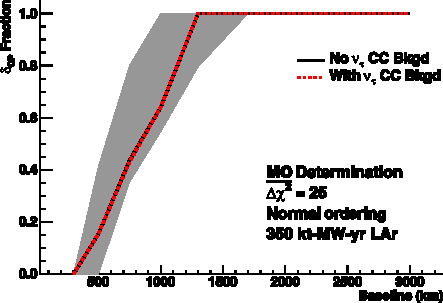
\includegraphics[width=\textwidth,keepaspectratio]{bass_MO.pdf}
          \end{subfigure}\hfill
          \begin{subfigure}[t]{0.49\textwidth}
            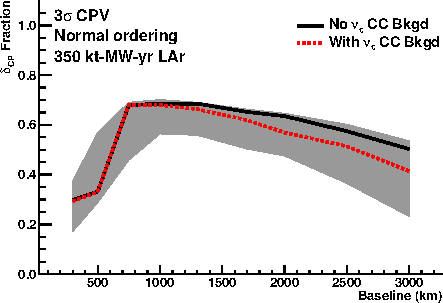
\includegraphics[width=\textwidth,keepaspectratio]{bass_cp.pdf}
          \end{subfigure}
            \caption[Détermination de l'ordre des masses et de la violation de CP en fonction de la ligne de base]{\label{fig::bass_fig}Graphes tirés de \cite{Bass2013}. Fraction des valeurs possibles de $\delta_{CP}$ auxquelles peut être déterminé l'ordre des masses avec 99.38\,\% de chance (gauche) et la violation de CP à $3\sigma$ (droite) en fonction de la ligne de base. L'ordre des masses est supposé normal et inconnu. La zone grisée montre la plage des valeurs possibles due aux incertitudes sur les autres paramètres des oscillations.}
        \end{figure}
        La ligne de base de \SI{1300}{\kilo\meter} suit une étude de simulation menée par M.Bass et.al. en 2013\cite{Bass2013}, dont le but était de déterminer la ligne de base optimale permettant de déterminer sans ambiguïtés l'ordre des masses et la violation de CP. Leurs simulations ont calculé, pour des lignes de bases comprises entre \SI{300}{\kilo\meter} et \SI{3000}{\kilo\meter}, le nombre attendu d'événements $\nu_e$ en fonction de l'énergie reconstruite dans un détecteur de \SI{50}{\kilo\tonne} d'argon liquide après 6 ans de prise de données, avec un faisceau initial de proton de \SI{1.2}{\mega\watt} et \SI{120}{\giga\electronvolt} ce qui correspondra au faisceau de \gls{dune} après la mise à niveau PIP-II. Le tout correspond alors à une exposition de \SI{350}{\kilo\tonne\mega\watt\year}. Pour chaque ligne de base, le faisceau était optimisé afin de couvrir les deux premiers maxima de probabilité de transition. Les auteurs ont inclue des estimations des bruits de fond les plus importants et se sont basés sur les études d'\gls{icarus}\cite{ref_needed} pour estimer les performances du détecteur. Ils génèrent des événements neutrinos et antineutrinos en supposant un temps d'exposition égal pour les deux, puis réalisent un ajustement combiné des spectres d'apparition des $\nu_e$ et de disparition des $\nu_{\mu}$. Les paramètres connus de la matrice \gls{pmns} étaient contraints à leur incertitudes expérimentales, les trois inconnues $\delta_{CP}$, l'ordre des masses et l'octant de $\theta_{23}$ étaient laissées libres. Une minimisation du $\chi^2$ est utilisée afin de déterminer ces trois paramètres. Les graphs de la \autoref{fig::bass_fig}, tiré de l'article de M.Bass et.al., montrent la fraction des valeurs possibles de $\delta_{CP}$ auxquelles il est possible de déterminer la violation de CP, l'ordre des masses et l'octant de $\theta_{23}$, en fonction de la ligne de base.

        Cette étude indique qu'une ligne de base d'au moins \SI{1300}{\kilo\meter} est nécessaire pour atteindre 99.38\,\% de chances de déterminer l'ordre des masses (avec l'analyse décrite dans \cite{Qian2012}) pour toutes les valeurs possibles de $\delta_{CP}$. Une ligne de base supérieure à \SI{700}{\kilo\meter} est requise pour atteindre une précision de $3\sigma$ sur la valeur de $\delta_{CP}$ pour un maximum de ses valeurs (70\,\%). Une ligne de base supérieure à \SI{1500}{\kilo\meter} entraîne une diminution de la fraction de $\delta_{CP}$ permettant d'atteindre ces $3\sigma$. La détermination de l'octant de $\theta_{23}$ à $5\sigma$ est possible pour toutes les valeurs de $\delta_{CP}$ au delà d'une ligne de base de à \SI{1000}{\kilo\meter}. Une ligne de base entre \SI{1200}{\kilo\meter} et \SI{1500}{\kilo\meter} est alors la meilleure option. L'existence du site de Sanford, à \SI{1300}{\kilo\meter} du Fermilab, à déterminé le choix de la ligne de base de \gls{dune}.
        
      \subsubsection{Le choix de la gamme d'énergies :}

        \begin{figure}[htpb]
          \begin{subfigure}[t]{0.49\textwidth}
            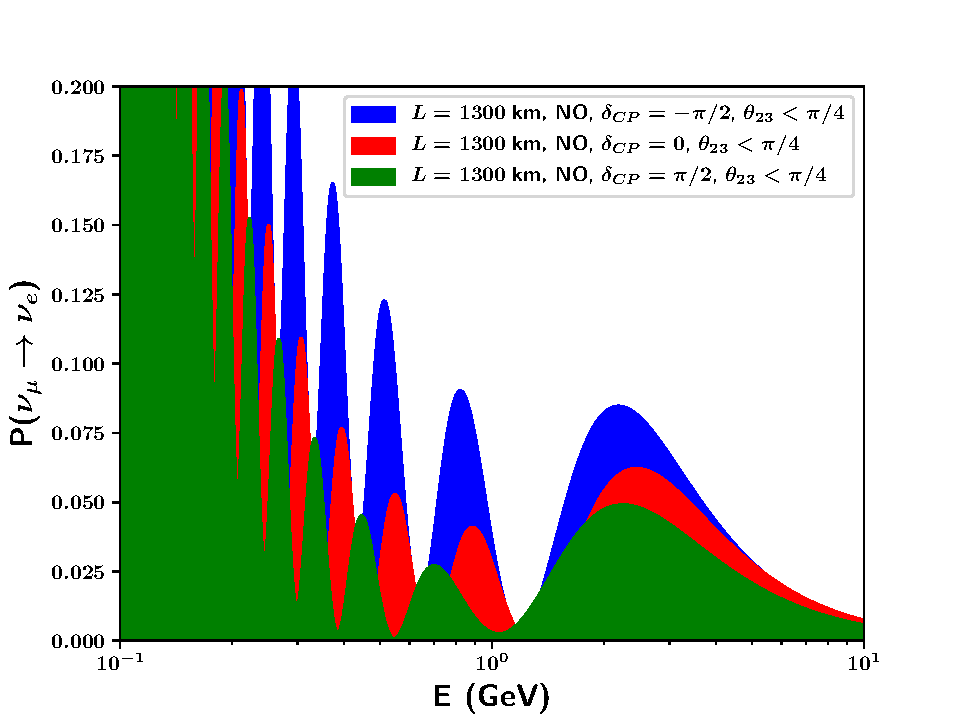
\includegraphics[width=\textwidth,keepaspectratio]{numu-nue-vs-E-cp.pdf}
          \end{subfigure}\hfill
          \begin{subfigure}[t]{0.49\textwidth}
            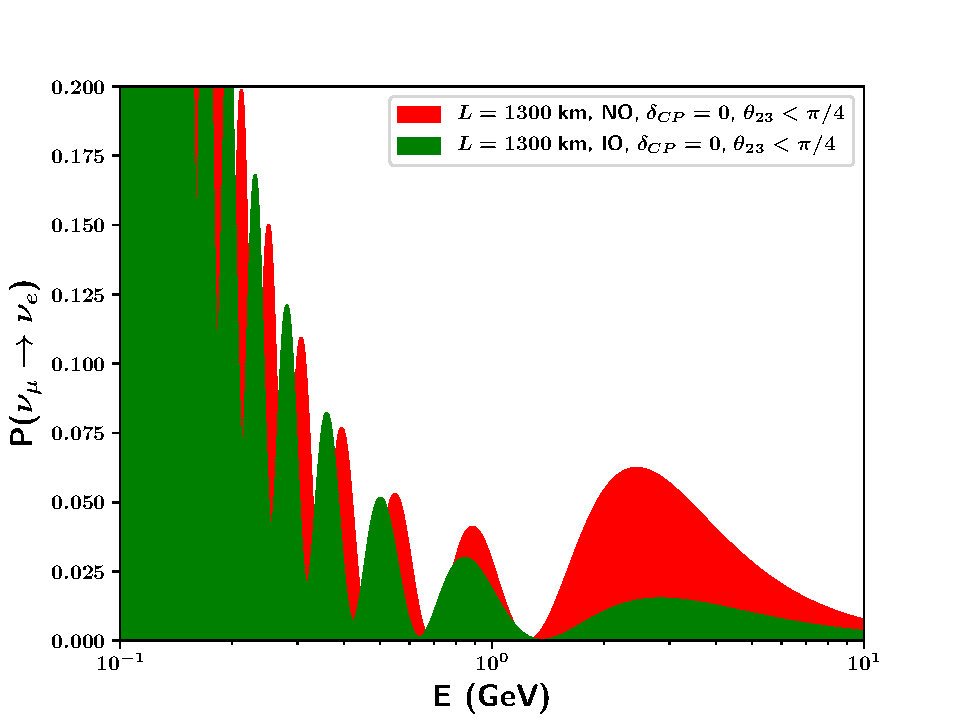
\includegraphics[width=\textwidth,keepaspectratio]{numu-nue-vs-E-MH.pdf}
          \end{subfigure}
            \caption[Probabilité de changement de saveur en fonction de $E$ à \SI{1300}{\kilo\meter}]{\label{fig::two_unknown_effects}Probabilité de changement de saveur en fonction de $E$ à \SI{1300}{\kilo\meter}. Le graphe de gauche montre l'impact de l'ordre des masses, avec $\delta_{CP}=0$. Le graphe de droite montre l'impact de $\delta_{CP}$, avec un ordre des masses normal.}
        \end{figure}
        La \autoref{fig::two_unknown_effects} montre les effets attendus de $\delta_{CP}$ et de l'ordre des masses sur $P(\nu_{\mu}\to\nu_e)$ en fonction de $E$ à la ligne de base de \gls{dune}. On peut voir que l'effet de la phase de violation de CP est plus important pour les maxima de probabilité aux énergies inférieures à \SI{1.5}{\giga\electronvolt}, ce qui correspond aux second et plus maxima de probabilité de transition. L'ordre des masses quant à lui est plus important au premier maximum. C'est pour cela que le faisceau de \gls{dune} sera compris entre  \SI{0.5}{\giga\electronvolt} et \SI{5}{\giga\electronvolt} : il permettra ainsi de couvrir les deux premiers maxima de probabilité d'oscillation et de séparer les effets de la violation de CP et des effets de matière.


    \subsection{Sensibilités attendues}\label{sec::sensibility}

        \gls{dune} mesurera $P\left(\nuanu_{\mu}\to\nuanu_e\right)$ et $P\left(\nuanu_{\mu}\to\nuanu_{\mu}\right)$ en fonction de l'énergie des neutrinos incidents afin de sonder l'ordre des masses et la violation de CP. Ces mesures seront faites en comptant le nombre d'interactions vues dans le détecteur et en estimant le nombre de (anti)neutrinos initialement générés par le faisceau. Seules les interactions par courant chargé ($CC$) pourront contribuer au signal : elles permettent de connaître la saveur du neutrino ayant interagit en identifiant la saveur du (anti)lepton chargé produit dans l'état final. Les interactions courant neutre ($NC$) ne permettent pas d'identifier la saveurs du (anti)neutrino car n'importe quel (anti)neutrino peut produire n'importe quel (anti)lepton via courant neutre. Ces interactions, ainsi que les interactions d'éventuels (anti)neutrinos tauiques, peuvent cependant créer des événements ressemblant aux interactions par courant chargé, soit en émettant un (anti)électron ou un (anti)muon dans l'état final (c'est le cas des interactions $\nuanu_{\tau} CC$), soit en produisant un $\pi^{\pm}$ ou un photon pouvant imiter respectivement un (anti)muon ou un (anti)électron.

        Les études des sensibilités de \gls{dune} sont tirées du second volume du CDR de 2015\cite{Collaboration2015}. La sensibilité à l'ordre des masses correspond à la probabilité qu'à \gls{dune} de déterminer si l'ordre est normal ou inversé. La sensibilité à la violation de CP correspond à la précision avec laquelle \gls{dune} pourra déterminer si $\delta_{CP} \neq 0$ ou $\pi$. Si $\delta_{CP} = 0$ ou $\pi$, alors la précision tombe naturellement à zéro. %La sensibilité à l'octant de $\theta_{23}$ correspond à la précision avec laquelle \gls{dune} pourra déterminer si $\theta_{23}>\pi/4$ ou $\theta_{23}<\pi/4$. Si $\theta_{23}=\pi/4$, alors la précision tombe naturellement à zéro également.

        \begin{figure}[htbp]
          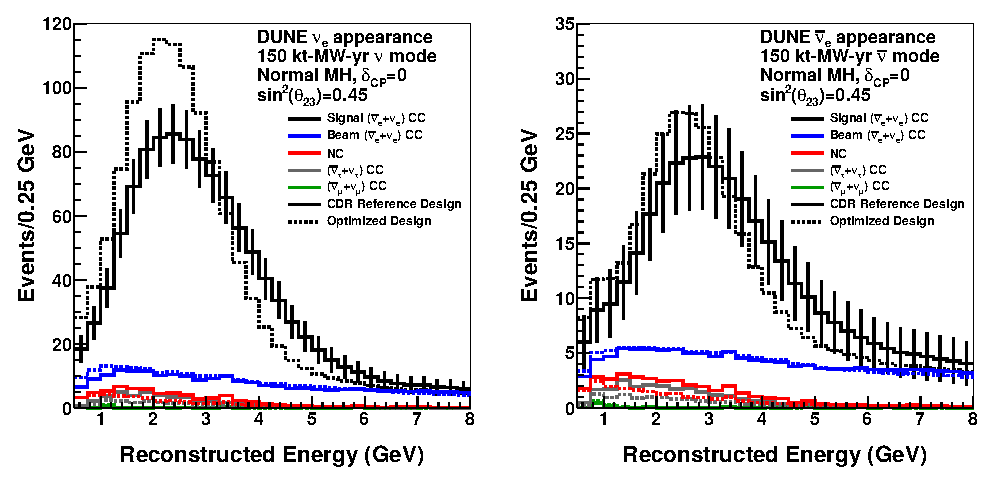
\includegraphics[width=\textwidth]{spectra.pdf}
          \caption[Distribution de l'énergie des événements attendus dans \acrshort{dune}]{\label{fig::spectra}Graphes tirés de \cite{Collaboration2015}. Distribution de l'énergie des événements d'apparition $\nu_e$ (gauche) et $\anu_e$ (droite) attendus dans \acrshort{dune} au bout de 7 ans de prise de données (3 ans et demi avec des neutrinos et autant avec des antineutrinos). Les événements sont sélectionnés en identifiant les interactions $\nuanu_e CC$ et contiennent donc du bruit de fond (lignes colorées). Les traits pleins correspondent au faisceau de référence et les traits pointillés au faisceau optimisé.}
        \end{figure}

        Pour évaluer la sensibilité de \gls{dune} à l'ordre des masses et à la violation de CP, une simulation est réalisée avec GLoBES\cite{ref_needed}, qui prend en entrée les données du flux du faisceau, les différentes sections efficaces et la réponse du détecteur (estimée avec une simulation Monte Carlo). La simulation des dépôts d'énergie et de l'identification des saveurs des neutrino permettent de générer les distributions d'énergie attendues. Dans cette simulation, le temps d'exposition est le même pour le faisceau de neutrino et le faisceau d'antineutrino. La \autoref{fig::spectra} montre un exemple d'une telle distribution (ou spectre) pour les 4 canaux $\nu_e CC$, $\nu_{\mu} CC$, $\anu_e CC$ et $\anu_{\mu} CC$. Un ajustement est fait simultanément sur ces 4 spectres. Dans cet ajustement, les paramètres des oscillations des neutrinos sont autorisés à varier dans un intervalle de $1\sigma$ gaussien autour de leur valeur moyenne. Les tailles de ces intervalles et les moyennes de ces paramètres sont fixées par les résultats d'un ajustement global sur les données d'oscillations de 2014\cite{ref_needed}. Les incertitudes systématiques (voir plus loin dans le texte) sont considérées comme 100\,\% décorrélées entre les 4 canaux.

        La sensibilité est définie par le test statistique $\Delta \chi^2$, calculé en comparant les spectres en énergie prédits pour différentes hypothèses. Pour évaluer la sensibilité à l'ordre des masses, les spectres sont générés en fixant l'ordre des masses sur une des deux possibilités (normale ou inversé). Cet ordre des masses est appelé "vrai" ordre. L'ajustement est alors fait sur les spectres des 4 canaux en supposant l'ordre des masses normal, puis inversé, indépendamment du choix fait pour généré les événements. Le test statistique est alors défini comme la différences entre les deux $\chi^2$ ainsi obtenus. Pour un "vrai" ordre des masses normal, on défini
        $$\Delta \chi^2_{MO}=\chi^2_{IO}-\chi^2_{NO},$$
        où $IO$ désigne l'ordre inversé et $NO$ l'ordre normal ($MO$ signifie "mass ordering"). L'opération est refaite en changeant le "vrai" ordre des masses. Pour un "vrai" ordre des masses inversé, on défini
        $$\Delta \chi^2_{MO}=\chi^2_{NO}-\chi^2_{IO}.$$
        Ces deux tests statistiques doivent être calculés pour toutes les valeurs de $\delta_{CP}$ et pour les deux octants possible de $\theta_{23}$. Pour la violation de CP, l'opération doit être réalisée pour l'ensemble des "vraies" valeurs possibles de $\delta_{CP}$, entre $0$ et $2\pi$. Pour chacune de ces "vraies" valeurs, l'ajustement est fait en supposant $\delta_{CP}^{test}=0$ puis $\delta_{CP}^{test}=\delta_{CP}^{true}$. Un test statistique intermédiaire est alors calculé et est défini par
        $$\Delta \chi^2_{CP}=\chi^2_{\delta_{CP}^{test}}-\chi^2_{\delta_{CP}^{true}}.$$
        Le calcul est refait avec $\delta_{CP}^{test}=\pi$\footnote{Si aucune fluctuation statistique n'est simulée, alors $\delta_{CP}^{true}=0$.}, puisque $0$ et $\pi$ sont les deux seules valeurs pour lesquelles il n'y a pas de violation de CP. Le test statistique sur la violation de CP $\chi^2_{CPV}$ est alors le minimum des deux tests intermédiaires. Comme ceci doit être fait pour toutes les valeurs de $\delta_{CP}^{true}$, $\chi^2_{CPV}$ est fonction de $\delta_{CP}^{true}$. Ce test est calculé pour les deux ordres des masses possibles et des deux octant possibles de $\theta_{23}$.%Le test statistique pour l'octant de $\theta_{23}$ est défini comme $$\Delta \chi^2_{octant}=|\chi^2_{\theta_{23}^{test}>\pi/4}-\chi^2_{\theta_{23}^{test}<\pi/4}|.$$ Comme $\delta_{CP}$, $\theta_{23}$ est continue est $\Delta \chi^2_{octant}$ sera fonction de $\theta_{23}$.
        
        Pour l'ordre des masses, une valeurs de $\sqrt{\Delta \chi^2}=3$ correspond à une probabilité de \numprint{98.9}\,\%
        %CDR vol 2 page 25(39) 
        de déterminer correctement l'ordre des masses. Une valeurs de $\sqrt{\Delta \chi^2}=5$ correspond à une probabilité de \numprint{99.9996}\,\%\cite{Collaboration2015}. Dans le cas de la violation de CP, $\sqrt{\Delta \chi^2}$ correspond à la précision à laquelle elle peut être déterminée et est égal à $\sigma$ ($3\sigma = 99.7\,\%$ et  $5\sigma = 99.9999\,\%$ de précision).
        
        Ces sensibilités sont contraintes par un certain nombre d'incertitudes systématiques:
        \begin{itemize}
          \item[$\bullet$] Des incertitudes sur le nombre d'événements attendus, aussi appelées incertitudes de normalisation (elles influencent le nombre d'événements mesurés). Ces dernières sont dues aux incertitudes sur le flux incidents, sur les sections efficaces des réactions de signal et de bruit de fond et sur les différents modèles d'interactions. Le détecteur proche pourra contraindre un certain nombre de ces systématiques en mesurant le flux et les sections efficaces avant que les neutrinos n'aient pu changer de saveur. En plus de cela, les expériences du programme \gls{sbn} du Fermilab mesurent avec précision les sections efficaces et les modèles d'interaction des neutrinos dans l'argon liquide. L'expérience \gls{argoneut}\cite{Anderson2012} a pris des donnée entre 2009 et 2010, \gls{microboone}\cite{Collaboration2016} en prend depuis 2015. Les détecteurs \gls{icarus}\cite{Farnese2011} et \gls{sbnd}\cite{Tufanli2017} commenceront leur prise de donnée en 2019 et 2020 respectivement. La \autoref{fig::normsigma_effect} montre les effets de ces incertitudes sur la sensibilité de \gls{dune} à la violation de CP. Ces effets attendus permettent de fixer les caractéristiques requises pour le faisceau, le détecteur proche et le détecteur lointain (décrits dans les prochaines sections) afin d'atteindre la précision requise de $5\,\%\oplus2\,\%$. 5\,\% est la précision sur la normalisation du spectre des $\nuanu_{\mu}$ vu par le détecteur lointain, et 2\,\% est la précision sur la normalisation du spectre des $\nuanu_e$ vu par le détecteur lointain.
          \item[$\bullet$] Des incertitudes sur l'énergie des neutrinos, aussi appelées incertitudes de forme (elles influencent la distribution en énergie des événements mesurés). Elles sont essentiellement dues aux imprécisions sur la reconstruction de l'énergie des neutrinos. Les expériences \gls{lariat}\cite{Nutini2017}, \gls{captain}\cite{Bian2015} et protoDU$\nu$E\cite{Manenti2017} étudient les interactions de particules chargées dans l'argon liquide afin de prédire au mieux les capacités du détecteur lointain à reconstruire cette énergie. Les effets de ces incertitudes sur les sensibilités sont encore en étude.
        \end{itemize}
         Les résultats montrés ici vont être améliorés dans le CDR 2019 après des études plus poussées des effets des différentes incertitudes (notamment de forme) sur les sensibilités, en prenant en compte les corrélations entre les incertitudes des données neutrinos et antineutrinos et les corrélations entre les 4 canaux.

        Les sensibilités sont également contraintes par la quantité de données que nous sommes en mesure d'accumuler. Cette quantité dépendra directement du flux de neutrinos. Dans le volume 3 du CDR\cite{Strait2016}, deux simulations GEANT4 du faisceau sont décrites : la première se base sur le faisceau de référence présenté en \autoref{sec::faisceau} et dans le volume 3 du CDR\cite{Strait2016}, dont le design est basé sur le faisceau déjà existant NuMI. La seconde utilise une version optimisée du faisceau, obtenue grâce à un algorithme génétique qui a cherché à maximiser le flux de neutrinos au détecteur lointain en faisant varier 20 paramètres du faisceau, intervenant dans l'impulsion initiale des protons, les dimensions et positions des différents éléments du faisceau et du courant dans les cornes magnétiques (voir \autoref{sec::faisceau}). Comparée au faisceau de référence, cette optimisation permet de créé un flux de neutrinos au détecteur lointain 20\,\% supérieur aux énergies du premier maximum de probabilité de transition (entre \SI{1.5}{\giga\electronvolt} et \SI{4}{\giga\electronvolt}) et 53\,\% supérieur aux énergies des second et plus maxima (entre \SI{0.5}{\giga\electronvolt} et \SI{1.5}{\giga\electronvolt}). Le tableau \autoref{tab::carac_beam} présente les principales caractéristiques du faisceau de référence et du faisceau optimisé.

        \begin{table}[htpb]
          \centering
          \begin{tabular}{|lcc|}
            \hline
            \textbf{Paramètre} & \textbf{Référence} & \textbf{Optimisé} \\ \hline\hline
            Énergie du faisceau de proton & \SI{80}{\giga\electronvolt} & \SI{80}{\giga\electronvolt} \\
            Puissance du faisceau de proton & \SI{1.07}{\mega\watt} & \SI{1.07}{\mega\watt} \\
            Cible & Graphite & Graphite  \\
            Courant dans les cornes & \SI{230}{\kilo\ampere} & \SI{297}{\kilo\ampere} \\
            Design des cornes & NuMi-style & Optimisation génétique \\
            Longueur du tuyau de désintégration & \SI{204}{\meter} & \SI{241}{\meter} \\
            Diamètre du tuyau de désintégration & \SI{4}{\meter} & \SI{4}{\meter} \\ \hline
          \end{tabular}
          \caption[Caractéristiques du faisceau de neutrino de \gls{dune}]{\label{tab::carac_beam}Principales caractéristiques du faisceau de neutrino qui sera envoyé depuis le Fermilab sur les détecteur lointain à Sanford. A gauche est présentée la version de référence, décrite en \autoref{sec::faisceau}. A droite est présentée la version obtenu par un algorithme génétique optimisant le flux de neutrinos au détecteur lointain.}
        \end{table}

        La \autoref{fig::sensitivities} présentent les sensibilités à l'ordre des masses et la violation de CP en fonction de l'exposition en \si{\kilo\tonne\mega\watt\year}. Dans les deux cas l'ordre des masses est supposé normal et inconnu. L'annexe \ref{annexe::sensitivity} montre ces sensibilités pour un ordre des masses inversé, et en fonction de $\delta_{CP}$ et de $\theta_{23}$. D'après ces graphes, un temps d'exposition de 7 ans avec une masse fiducielle de \SI{40}{\kilo\tonne} et un faisceau de \SI{1.07}{\mega\watt} (\SI{300}{\kilo\tonne\mega\watt\year}) correspond à \numprint{99.9996}\,\% de chance de déterminer l'ordre des masses à $5\sigma$ pour toutes les valeurs possibles de $\delta_{CP}$. La violation de CP peut être déterminée à $5\sigma$ pour \numprint{50}\,\% de ses valeurs après environ 13 ans, toujours avec une masse fiducielle de \SI{40}{\kilo\tonne} et un faisceau de \SI{1.07}{\mega\watt} (\SI{550}{\kilo\tonne\mega\watt\year}). $3\sigma$ pour \numprint{75}\,\% des valeurs de $\delta_{CP}$ sont atteint après environ 20 ans (\SI{850}{\kilo\tonne\mega\watt\year}).

        
        \begin{figure}[htbp]
          \begin{subfigure}[t]{0.43\textwidth}
            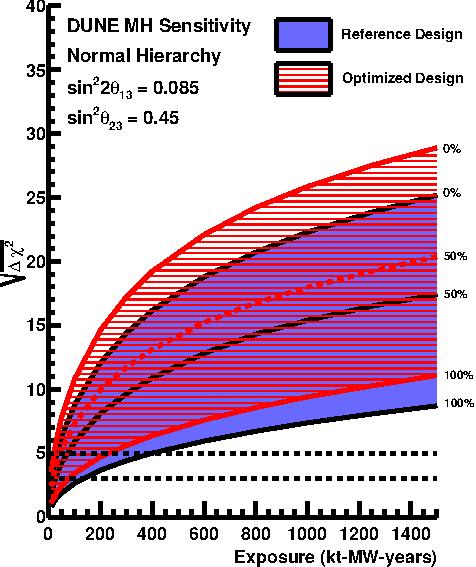
\includegraphics[width=\textwidth]{sensitivity_MH.pdf}
          \end{subfigure}\hfill
          \begin{subfigure}[t]{0.43\textwidth}
            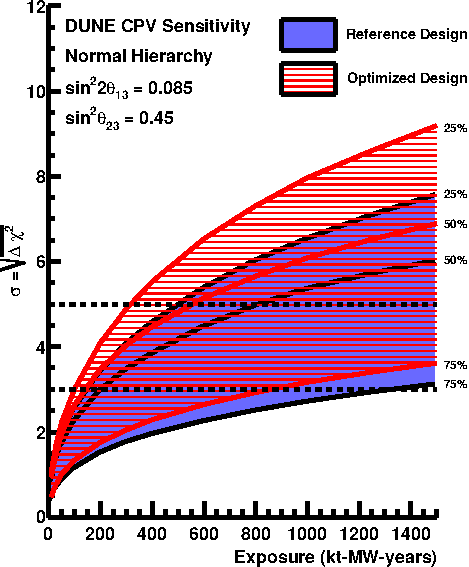
\includegraphics[width=\textwidth]{sensitivity_CP.pdf}
          \end{subfigure}
          \caption[Sensibilités attendues à l'ordre des masses et à la violation de CP]{\label{fig::sensitivities}Graphes tirés de \cite{Collaboration2015}. Sensibilités attendues à l'ordre des masses (gauche) et à la violation de CP (droite) en fonction de l'exposition, pour le faisceau de référence (en bleu plein) et le faisceau optimisé (en rouge hachuré). L'ordre des masses est supposé normal et inconnu.}
        \end{figure}

        \begin{wrapfigure}{R}{0.48\textwidth}
          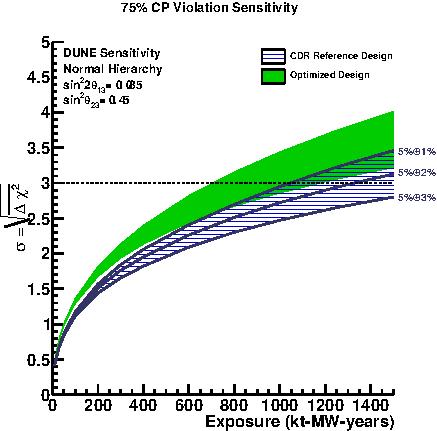
\includegraphics[width=0.48\textwidth]{sensitivity_norm_uncertainties.pdf}
          \caption[Effet des incertitudes de normalisation sur la sensibilité de \gls{dune}]{\label{fig::normsigma_effect}Graphes tirés de \cite{Collaboration2015}. Effet des incertitudes de normalisation sur la sensibilité à la violation de CP pour 75\,\% des valeurs de $\delta_{CP}$.}
        \end{wrapfigure}
        Afin d'atteindre ces sensibilités, le faisceau, le détecteur proche et le détecteur lointain doivent atteindre certaines performances\cite{Collaboration2015}. Le faisceau doit couvrir un spectre en énergie assez large pour permettre d'atteindre les deux premiers maxima de probabilité de transition, qui sont à \SI{2.4}{\giga\electronvolt} et \SI{0.8}{\giga\electronvolt} respectivement pour une ligne de base de \SI{1300}{\kilo\meter}. Il doit être capable de produire au choix un faisceau de neutrino muonique ou d'antineutrino muonique, avec une contamination de (anti)neutrinos électroniques aussi faible que possible.

        Le détecteur lointain doit être capable d'identifier les événements $\nuanu_e CC$ et $\nuanu_{\mu} CC$ précisément et en nombre suffisant, et de reconstruire l'énergie totale de ces événements. Il doit être capable d'identifier les gerbes électromagnétiques et hadroniques et de les contenir en entier dans son volume. Les événements dues aux rayons cosmiques ne doivent pas constituer plus de 1\,\% du total d'événements. Le détecteur doit donc être profondément enterré.

        Le détecteur proche doit pouvoir prédire le flux attendu au détecteur lointain avec suffisamment de précision pour que les erreurs systématiques associées soient négligeables en comparaison des erreurs statistiques sur toute la durée de l'expérience. Il doit pouvoir entre autre prédire le flux de $\nu_{\mu}$ avec une précision d'au plus 5\,\% et le flux de $\nu_e$ avec une précision d'au plus 2\,\%. Il doit pouvoir mesurer la contamination en $\nuanu_e$ du faisceau avant changement de saveur et étudier en détail la topologie des événements pouvant ressembler à du signal. Il doit pouvoir mesurer avec précision différentes sections efficaces en fonction de l'énergie du neutrino.
        %PLOTS CDR 2 PAGE 45
        %	         En effet, une expérience à longue ligne de base tire profit de l'effet MSW (voir \autoref{sec::MSW}) qui apparaît quand les neutrinos incidents traversent de la matière. Cet effet est directement sensible au signe de la différence de masse. Cependant, il induit une différence de comportement entre neutrinos et anti-neutrino qui peut masquer l'effet de $\delta_{CP}$, puisque les antineutrinos ne réagissent pas de la même manière que les neutrinos en présence de matière ordinaire. \gls{dune} mesurera la probabilité  $P(\nu_{\mu} \to \nu_e)$, décrite par l'équation \eqref{eq::proba_matter_3flavors}, en fonction de l'énergie du neutrino incident $E$. La probabilité $P(\overline{\nu}_{\mu} \to \overline{\nu}_e)$ en fonction de $E$ sera également mesuré en générant un faisceau d'antineutrinos. Pour passer de $P(\nu_{\mu} \to \nu_e)$ à $P(\overline{\nu}_{\mu} \to \overline{\nu}_e)$, il faut inverser les signes de $\delta_{CP}$ et $A$ dans l'équation \eqref{eq::proba_matter_3flavors}. Une asymétrie matière-antimatière se traduit par une dépendance en $E$ légèrement différente entre ces deux probabilités. La \autoref{fig::asym} montre les effets de $\delta_{CP}$ et de matière séparément sur ces deux probabilité.
        %	         %FAIRE LA FIGURE ET COMMENTER
        %	          Cette asymétrie peut être encodée dans la variable
        %	         \begin{equation}\label{eq::asym_var}
        %	         	\mathcal{A}_{CP}(E_{\nu}) = \frac{P(\nu_{\mu} \to \nu_e) - P(\overline{\nu}_{\mu} \to \overline{\nu}_e)}{P(\nu_{\mu} \to \nu_e) + P(\overline{\nu}_{\mu} \to \overline{\nu}_e)}
        %	         \end{equation}
        
        
        
        %	          dont dépendent un certain nombre de théories. \gls{dune} déterminera ces deux inconnues en mesurant la probabilité $P(\nu_{\mu \to \nu_e)$ décrite par l'équation \eqref{eq::proba_matter_3flavors}. La phase de violation de CP apparaît directement cette l'équation. L'ordre des masses sera connue quand le signe de  sera connu. Cette différence de masse peut être mise en évidence grâce à l'effet de résonance MSW (voir \autoref{sec::MSW}), qui apparaît quand les neutrinos oscillent dans la matière. Les effets de matières et l'effet de la phase de violation de CP créent tout deux une asymétrie entre le comportement des neutrinos et des antineutrinos.
  \section{\texorpdfstring{DU$\nu$E}{DUNE} : le faisceau et les détecteur proche et lointain}\label{sec::faisceau_et_det}

    \subsection{Le faisceau de neutrino}\label{sec::faisceau}

      Il existe trois principaux types de faisceau de neutrino :
      \begin{itemize}
        \item[$\bullet$] les faisceaux $\beta$, qui récupèrent les neutrinos issues de désintégrations $\beta$,
        \item[$\bullet$] les usines à neutrinos, qui récupèrent les neutrinos issues de la désintégrations de muons
        \item[$\bullet$] les faisceaux mésoniques, qui récupèrent les neutrinos issues de la désintégrations de méson.
      \end{itemize}
      Seul la dernière de ces trois technologies a déjà été utilisé pour des expériences, les deux premières étant encore en phase de prototypage. L'expérience \gls{dune} utilisera un faisceau mésonique, aussi nous nous concentrerons sur cette technologie dans la suite du texte. Pour plus d'informations sur les faisceaux $\beta$, le lecteur peut consulter l'article~\cite{Wildner2012}, et l'article~\cite{Bogomilov2014} pour plus d'informations sur les usines à neutrinos.
        
        %Le faisceau $\beta$, le plus récent des trois, est encore en phase de prototypage. Nous n'en parlons que rapidement, par soucis d'exhaustivité, car ce n'est pas la technologie employée dans \gls{dune}. Plus de détails sont consultables dans cet article~\cite{Wildner2012}. Il s'agit de produire et stocker des noyaux radioactifs se désintégrant via la désintégration $\beta$ puis de les collimater pour de les laisser se désintégrer et ainsi produire un faisceau de (anti)neutrino électronique. L'avantage de cette technologie est d'avoir un spectre en énergie très restreint et ajustable, possiblement de basse énergie permettant de placer un détecteur relativement proche de la source pour correspondre à un maximum de probabilité d'oscillation, limitant ainsi les effets de matière sur les oscillations. Ceci permet d'être plus sensible à la violation de CP qu'avec une expérience à longue ligne de base.
        
        %La seconde technologie de faisceau de neutrino est l'usine à neutrino. Comme pour le faisceau $\beta$, elle est en cours de développement et ne sera pas utilisé dans \gls{dune}, nous n'en parlons donc que rapidement, plus de détails se trouvant ici~\cite{Bogomilov2014}. Il s'agit de produire des mésons en projetant des protons sur une cible, de laisser ces mésons se désintégrer en muons et anti-muons qui sont stockés dans un anneau afin de les laisser se désintégrer à leur tour en neutrinos et anti-neutrinos électroniques et muoniques. L'avantage de cette technologie est de produire des faisceaux composés précisément de 50\% de neutrinos muonique et de 50\% de neutrinos électronique, contrairement à la technologie actuelle qui, comme décrit plus bas, produit des faisceaux avec environ 99\% de neutrinos muoniques et environ 1\% de contamination de neutrinos électroniques. En effet la connaissance précise de la composition en saveurs du flux de neutrino est primordiale pour effectuer des mesures d'oscillation de saveurs.
        
        %La troisième technologie, schématisée en \autoref{fig::faisceau}, est celle qui est utilisée actuellement dans les expériences d'oscillation de neutrinos d'accélérateurs à longue ligne de base, et qui est prévue pour \gls{dune}. 
      

      \begin{figure}[htbp]
        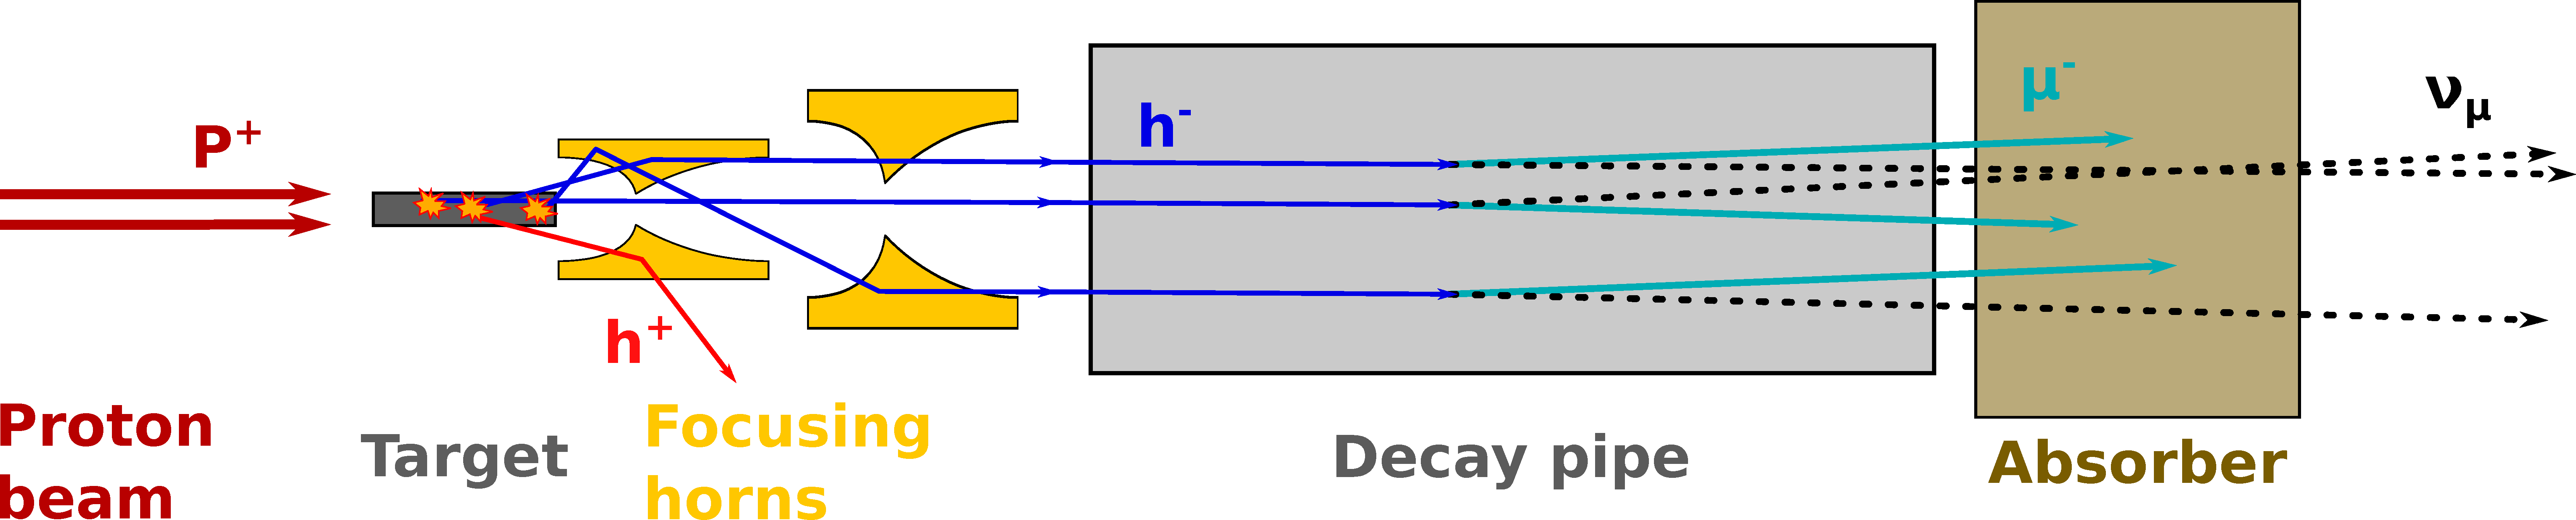
\includegraphics[width=\textwidth]{faisceau.pdf}
        \caption[Schéma de la création d'un faisceau de neutrinos]{\label{fig::faisceau}Schéma de la création d'un faisceau de neutrino. Un faisceau de proton ($P^+$) interagit dans une cible où sont produits, entre autre, des mésons chargés positivement ($h^+$) et négativement ($h^-$). Les cornes magnétiques dévient les mésons négatifs et focalisent les mésons positifs, qui se désintègrent en $\mu^+$ et $\nu_{\mu}$. Les $\mu^+$ sont stoppés dans l'absorbeur et les $\nu_{\mu}$ continuent.}
      \end{figure}
      \begin{figure}[htbp]
        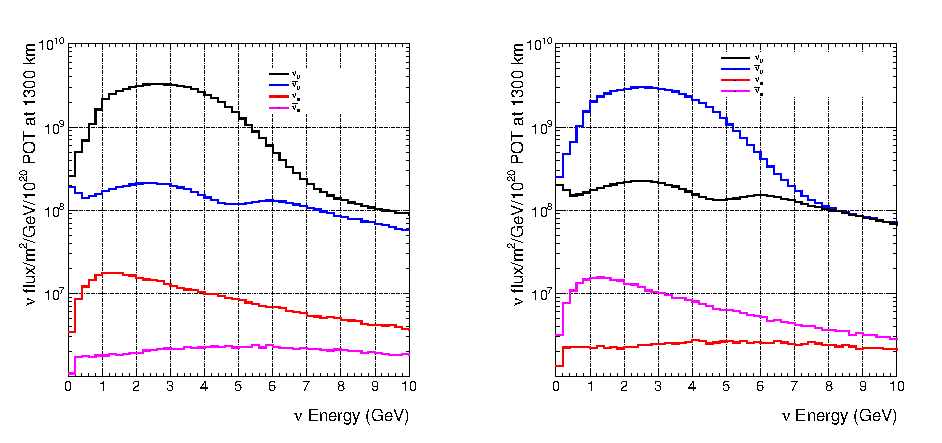
\includegraphics[width=\textwidth]{flux.pdf}
        \caption[Flux de neutrinos attendus sans oscillations au détecteur lointain de \gls{dune}]{\label{fig::flux}Flux de neutrinos (gauche) et antineutrinos (droite) électroniques et muoniques attendus en l'absence du phénomène d'oscillation des neutrinos au détecteur lointain de \gls{dune} avec le faisceau de référence.}
      \end{figure}
      La \autoref{fig::faisceau} est un schéma de la création d'un faisceau de neutrinos par désintégration de mésons. Il s'agit de produire des mésons chargés (essentiellement des pions et des kaons) en envoyant des protons sur une cible fixe, généralement du graphite. Ces mésons sont ensuite focalisés par une ou plusieurs cornes magnétiques, qui permettent également d'enlever les mésons chargés positivement ou négativement suivant que l'on cherche à produire un faisceau de neutrinos ou d'anti-neutrinos. Les mésons entrent ensuite dans un long tuyau pour s'y désintégrer en muons et neutrinos muoniques, avec une faible contaminations de neutrinos électronique due au canal de désintégration rare du kaon $K$ $K^+ \to e^+ \pi^0 \nu_e$. Si l'énergie est suffisante, il peut également y avoir une faible contamination en neutrinos tauiques due à la désintégrations de mésons $D_s$. Les mésons restant ainsi que les produits de désintégrations autres que les neutrinos sont arrêtés par une couche épaisse, en acier dans l'expérience \gls{dune}. Il est également possible de se passer de tuyau de désintégration et d'envoyer directement les mésons dans la roche ou le béton, afin qu'ils interagissent avant de se désintégrer. Les neutrinos viendront alors des produits de ces interactions à court temps de vie. Le faisceau résultant sera bien moins intense, mais sera composé d'autant de neutrinos que d'anti-neutrinos, électroniques et muoniques, ainsi que d'une fraction non négligeable de neutrinos et d'anti-neutrinos tauiques. Cette technique, appelée \textit{beam dump}, n'est pas utilisée dans \gls{dune}, qui cherche à avoir des neutrinos d'une seule saveur dans son faisceau.
        
      Les articles \cite{Levy2010,McDonald2001,Itow2001} montrent que le spectre en énergie attendue des neutrinos dépend de l'angle entre la direction de propagation du neutrino et l'angle principal du faisceau. Positionner un détecteur de manière légèrement désaxé (\SI{2.5}{\degree} pour l'expérience \gls{t2k} par exemple) permet non seulement de choisir le maximum du spectre à une énergie correspondant à un maximum de probabilité de transition, mais aussi d'avoir un spectre plus étroit. Dans \gls{dune}, l'idée est d'avoir un spectre assez large pour couvrir deux maxima de probabilité, aussi les détecteurs proche et lointain seront situés sur l'axe du faisceau.

      Les valeurs des différentes caractéristiques décrites ci-dessous correspondent au design de référence publié dans le volume 3 du CDR de 2015\cite{Strait2016} les possibles changements induit par l'optimisation de ce design sont présentés dans le \autoref{tab::carac_beam}.
        
      \paragraph{Le faisceau de proton de DU$\nu$E:} Le faisceau de proton servant à produire les neutrinos pour \gls{dune} sera créé par le complexe d'accélérateur du Fermilab, qui aura été mis à niveau et pourra fournir une puissance de $\SI{1.2}{\mega\watt}$ pendant les cinq premières année. Une seconde mise à niveau pourra monter cette puissance à $\SI{2.4}{\mega\watt}$ d'ici 2030. Il fonctionnera par cycle, produisant chacun \numprint{7.5e13} protons dont l'énergie peut varier de $\SI{60}{\giga\electronvolt}$ (cycle de \SI{0.7}{\second} et puissance de $\SI{1.2}{\mega\watt}$)  à $\SI{120}{\giga\electronvolt}$ (cycle de \SI{1.2}{\second} et puissance de $\SI{1.03}{\mega\watt}$). En générant un faisceau d'un certain signe (neutrinos ou antineutrinos), diminuer l'énergie des protons incidents augmente le flux du signe voulu à basse énergie et diminue la contamination de l'autre signe, améliorant légèrement la sensibilité. En dessous de $\SI{60}{\giga\electronvolt}$ des contraintes techniques baisse drastiquement la sensibilité\cite{Collaboration2015}. Les prédictions présentées dans cette section sont faites en supposant une énergie de $\SI{80}{\giga\electronvolt}$, correspondant à une puissance de $\SI{1.07}{\mega\watt}$.
        
      \paragraph{La cible:} Les protons iront frapper une cible longue de $\SI{95}{\centi\meter}$ faite de 47 segments de graphites, où 85\,\% des protons interagiront pour produire en majorité des pions et des kaons. 
        
      \paragraph{Les cornes magnétiques:} Imaginées par S.Van Der Meer en 1961\cite{VanDerMeer1961}, une corne magnétique agit sur les particules chargées comme une lentille peut agir sur la lumière. Elle consiste en deux conducteurs de symétrie axiale, un intérieur et un extérieur. Un courant entre par le conducteur intérieur et ressort par le conducteur extérieur, créant un champ magnétique entre les deux conducteurs. Les particules d'un signe de charge électrique donné produites dans la cible sont libres de traverser le conducteur intérieur -- qui doit être assez fin pour ne pas en absorber trop et assez épais pour supporter les forces magnétiques -- et seront ensuite déviées pour être parallèles à l'axe de la corne par le champ magnétique. Les particules de signe opposé seront déviées vers l'extérieur de la corne et s'en échapperont. Changer le sens du courant change le signe focalisé, et permet de choisir entre neutrinos et antineutrinos. \gls{dune} sera muni de deux cornes magnétique dont les conducteurs intérieurs ont une géométrie parabolique. L'article \cite{Kopp2006} résume les différentes géométries possibles et leurs intérêts. Les cornes paraboliques sont capables de focaliser les pions d'une impulsion données pour n'importe quel angle incident. Une seconde corne permet d'améliorer la focalisation, en récupérant les particules trop ou trop peu focalisées par la première cornes. La \autoref{fig::faisceau} montre un exemple de faisceau utilisant deux cornes paraboliques. Dans \gls{dune}, les 50 derniers centimètres de la cible sont dans la première corne magnétique, longue de $\SI{3.36}{\meter}$ et large de $\SI{16.5}{\centi\meter}$. Elle sera parcourue par un courant de $\SI{230}{\kilo\ampere}$. L'entrée de la seconde corne est située à $\SI{3.24}{\meter}$ de la sortie de la première corne. Cette seconde corne, parcourue par le même courant, est longue de  $\SI{3.63}{\meter}$ et large de $\SI{39.5}{\centi\meter}$. Chacune des deux cornes est constituée de deux conducteurs, intérieurs et extérieur, faits en Aluminium Al~6061-T6. Les conducteurs extérieurs sont cylindriques, tandis que les conducteurs intérieurs sont fait de deux paraboles communiquant par une petite ouverture de $\SI{9}{\milli\meter}$ dans la première corne et de $\SI{39}{\milli\meter}$ dans la deuxième. Les dimensions des cornes (longueur, diamètres extérieur et intérieur, distances à la cible et distance entre les cornes) vont avoir un impact important sur le spectre en énergie du flux de neutrinos.
        %Détailler windows?
        
      \paragraph{Le tuyau de désintégration:} $\SI{17}{\meter}$ après la sortie de la seconde corne se trouve l'entrée du tuyau de désintégration d'un diamètre de $\SI{4}{\meter}$, long de $\SI{194}{\meter}$ et rempli d'hélium, où les mésons pourront se désintégrer et produire les neutrinos. Ce tuyau est pointé vers le bas, avec une pente de 10\,\%.
        
      \paragraph{L'absorbeur:} A la fin du tuyau de désintégration se trouve la cavité contenant l'absorbeur, à $\SI{30}{\meter}$ sous la surface. C'est un assemblage d'aluminium, d'acier et de béton, où les particules chargées restantes seront arrêtées. A cet endroit se trouve aussi une alcôve à muons dont le but est de détecter les muons produits avec les neutrinos lors des désintégrations des mésons. En effet, ces muons nous donnent une information sur la direction, l'intensité, le flux et la largeur du faisceau, qu'il sera important de surveiller durant les opérations.
        
      \paragraph{Le flux:} Les neutrinos issues de ce faisceau auront des énergies comprises entre $\SI{0.5}{\giga\electronvolt}$ et $\SI{5}{\giga\electronvolt}$. Au niveau du détecteur lointain, $\SI{1300}{\kilo\meter}$ plus loin, les pics de probabilité de transition correspondront à des énergies de $\SI{0.8}{\giga\electronvolt}$ et $\SI{2.4}{\giga\electronvolt}$, qui sont donc comprises dans le spectre du faisceau de neutrinos. Les flux attendues sans oscillations au niveau du détecteur lointains sont présentés en \autoref{fig::flux}.

      \paragraph{Le faisceau optimisé:} Comme mentionné en début de section, des simulations ont été faites afin de trouver des valeurs des caractéristiques du faisceau décrites plus haut améliorant le flux au détecteur lointain. Le \autoref{tab::carac_beam} résume les différences entre le faisceau de référence et le faisceau optimisé. La \autoref{fig::spectra} montre les spectres en énergie des événements neutrinos courant chargé attendus au niveau de détecteur lointain pour ces deux designs, et la \autoref{fig::sensitivities} montre que le design optimisé améliore la sensibilité à l'ordre des masses et à la violation de CP.
        
    \subsection{Le détecteur proche}\label{sec::near_detector}
        %\cite{Meloni2018}

      \begin{figure}[htbp]
        \centering
        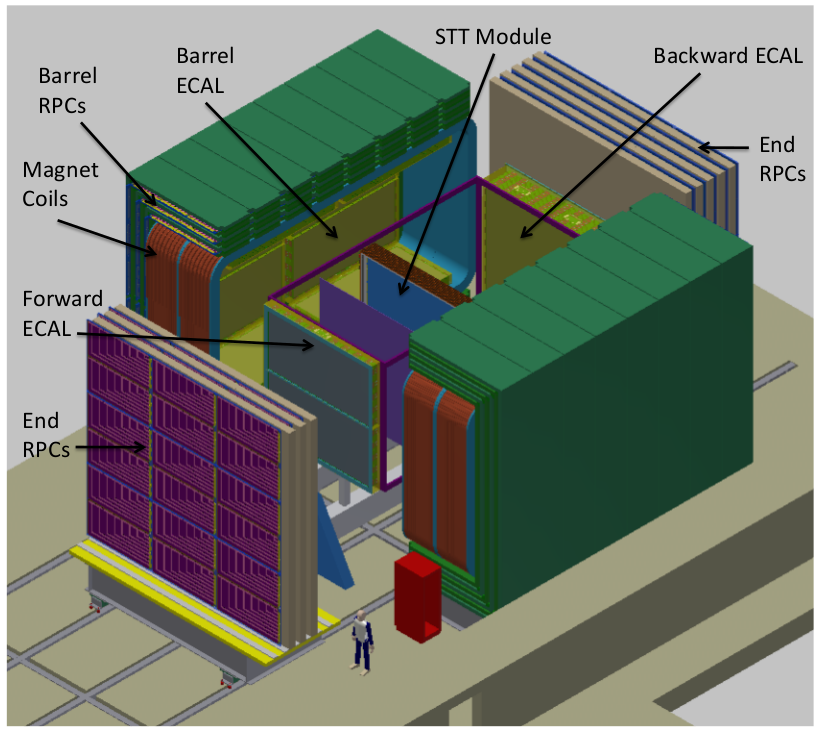
\includegraphics[width=0.8\textwidth]{ND.png}
        \caption[Schéma du détecteur proche de \gls{dune}]{\label{fig::ND}Schéma du détecteur proche de \gls{dune}.}
      \end{figure}
      Après l'absorbeur, le faisceau est constitué uniquement de (anti)neutrinos. La majorité seront muoniques, avec une faible composante de (anti)neutrinos électroniques. Le faisceau continue en ligne droite jusqu'au détecteur proche, situé \SI{300}{\meter} après l'alcôve à muons. Le détecteur proche mesurera en détails le spectre en énergie et la composition en saveurs ($\nuanu_e$, $\nuanu_{\mu}$ et $\nuanu_{\tau}$) du faisceau ainsi que les sections efficaces d'interaction courant chargé et courant neutre, afin de réduire les erreurs systématiques lors du comptage des événements au détecteur lointain, et ainsi d'atteindre une précision suffisante à la détermination de l'ordre des masses et de la violation de CP. Il sera magnétisé afin de déterminer la charge des leptons dans l'état final d'une réaction (anti)neutrino, permettant de faire facilement la différence entre une interaction neutrino et une interaction antineutrinos. Le détecteur proche servira aussi à collecter des données d'interaction neutrinos en grande quantité, permettant un programme de recherche lui étant propre, allant de la mesure de précision de processus électrofaible à des tests de physique au delà du modèle standard\cite{Collaboration2015}.

      Le détecteur proche sera un trajectographe à grain fin capable de reconstruire efficacement des protons à partir de \SI{250}{\mega\electronvolt\per c}, technologie ayant fait ses preuves avec l'expérience NOMAD\cite{Vannucci2014}. Il s'agira d'un module central de trajectographe composé de \numprint{107520} tubes de dérive de \SI{1}{\centi\meter} de diamètre et \SI{3.5}{\meter} de long. Ces tubes seront rempli d'un mélange de gaz argon-CO$_2$ et assemblés en 80 modules (STT) de $350\times350\times\SI{8.0}{\centi\meter\cubed}$ (pour un longueur totale de \SI{6.4}{\meter}) comportant des tubes verticaux et des tubes horizontaux. Entre chaque couche de tubes seront placées les cibles où les neutrinos interagiront. Il s'agira de feuilles de polypropylène de $\SI{25}{\micro\meter}$ d'épaisseur, 240 par modules, représentant plus de 80\,\% de la masse totale de chaque module. En plus des cibles en polypropylène, des cibles composés de différents matériaux (fer, carbone, calcium, eau,  eau lourde et argon) seront situées devant le trajectographe afin de réaliser des mesures d'interactions neutrinos sur ces différents noyaux cibles. La cible d'argon gazeux permettra d'extrapoler les mesures du détecteur proche au détecteur lointain et devrait être capable d'accumuler 10 fois plus de statistiques en terme d'interaction neutrinos que le détecteur lointain de \SI{40}{\kilo\tonne} d'argon liquide.

      Le trajectographe sera entouré à l'avant, à l'arrière et sur les côtés de \glspl{ecal} à échantillonnage. Il sera composé d'absorbeurs en plomb et de barres de scintillateurs plastiques de $\SI{3.2}{\meter}\times\SI{2.5}{\centi\meter}\times\SI{1}{\centi\meter}$ alternativement horizontales et verticales, capables de reconstruire électrons, positrons et photon avec une résolution en énergie inférieure à $6\,\%/\sqrt{E}$ (\si{\giga\electronvolt})\cite{Bhuyan2017}. 

      Le trajectographe et les 4 modules des \glspl{ecal} résideront dans un champ magnétique de $\SI{0.4}{\tesla}$ servant à l'identification de la charges des particules chargées et à la mesure des impulsions. Il sera généré par deux aimants situés à droite et à gauche du trajectographe (voir \autoref{fig::ND}). 

      Des identificateurs de muon entoureront chaque aimant, capables de différencier les muons des hadrons puisque ces derniers produiront des gerbes dans le fer, contrairement aux muons. Ces identificateurs permettront la reconstruction des trajectoires des muons à partir des traces vues par le trajectographe. Ils seront constitués de 432 \glspl{rpc} entrecoupées par l'acier des pôles magnétiques. 

      Les performances attendues du détecteur proche sont résumées dans le \autoref{tab::ND-perf}.

      \begin{table}[htpb]
        \centering
        \begin{tabular}{|lr|}
          \hline
          \textbf{Paramètre}                         & \textbf{Incertitude} \\ \hline
          Flux absolu de neutrino  & $\simeq 2.5$\,\%   \\
          Ratio des compositions $\nu_e/\nu_{\mu}$          & $< 1$\,\%        \\
          Ratio des compositions $\anu_e/\anu_{\mu}$      & $\simeq 1$\,\%     \\ \hline
        \end{tabular}
        \caption[Précision du détecteur proche]{\label{tab::ND-perf}Précision avec laquelle le détecteur proche pourra contraindre le flux total de neutrinos et la composition en saveur des flux de (anti)neutrinos.}
      \end{table}
      %TDR vol 3 page 100

      \subsection{Le détecteur lointain}\label{sec::far_detector}

        \begin{figure}[htbp]
          \centering
          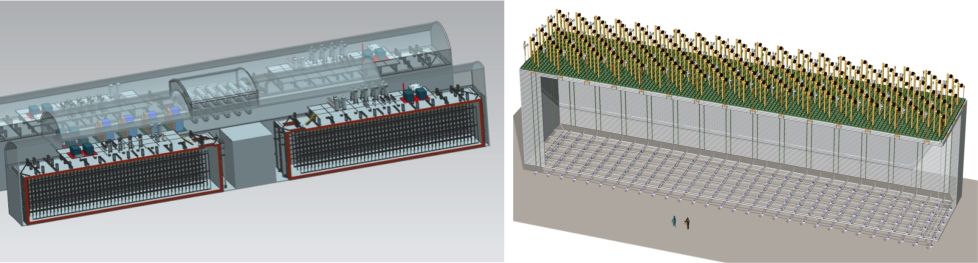
\includegraphics[width=\textwidth]{FD.pdf}
          \caption[Schéma du détecteur lointain de \gls{dune}]{\label{fig::FD}Schéma du détecteur lointain de \gls{dune}. Deux modules du design de référence sont à gauche, un module du design double phase est à droite.}
        \end{figure}
        Après avoir parcourue \SI{1300}{\kilo\meter} à travers la croûte terrestre, les neutrinos atteindrons le détecteur lointain, constitué de 4 modules contenant chacun \SI{10}{\kilo\tonne} d'argon liquide (voir \autoref{fig::FD}). Ils seront situés \SI{1450}{\meter} sous la surface afin d'être protégé des rayons cosmiques. Ce seront des \acrfull{lartpc}, dont la technologie est décrite en détail en \autoref{sec::lartpc}. Cette technologie offre une précision millimétrique, une très bonne résolution en énergie et une reconstruction 3D des interactions, le tout dans un seul élément homogène et dense, l'argon liquide. Le détecteur lointain permettra donc l'étude détaillée des interactions neutrinos. Bien que cette technologie ait déjà fait ces preuves avec les \SI{600}{\tonne} d'\gls{icarus}, un module de \SI{10}{\kilo\tonne} nécessite une étape de prototypage supplémentaire. Le projet protoDU$\nu$E au \gls{cern} a pour objectif de déterminer la faisabilité d'une \gls{lartpc} à l'échelle de \gls{dune}. Il étudie également une alternative, la \gls{dlartpc} avec le projet \gls{wa105}/protoDU$\nu$E-DP, dont la technologie est décrite en \autoref{sec::dlartpc}. Cette dernière permet d'amplifier les charges à détecter dans une fine couche d'argon gazeux en haut du volume de détection, et ainsi d'améliorer le rapport signal/bruit, offrant la possibilité de réduire le seuil de détection en énergie et ainsi de voir des événements de plus basse énergie. 

        Les performances requises et attendues de la version sans phase gazeuse du détecteur lointain sont résumées dans le \autoref{tab::FD-perf}.

        \begin{table}[htpb]
          \begin{tabular}{|l|ccc|}
            \hline
            \textbf{Paramètre} & \textbf{Requis} & \textbf{Atteint} & \textbf{Attendu} \\ \hline \hline
            Signal/Bruit & $9:1$ & $10:1$ & $9:1$ \\ 
            \specialrule{.01em}{.0em}{.0em}
            \begin{tabular}[c]{@{}l@{}}Incertitude sur l'atténuation de la charge \\  dans l'argon liquide\end{tabular} & $<5\,\%$ &  $<1\,\%$ &  $<1\,\%$\\
            \specialrule{.01em}{.0em}{.0em}
            Résolution de la position des vertex &  $(\numprint{2.5};\numprint{2.5};\numprint{2.5})\si{\centi\meter}$ &  & $(\numprint{1.1};\numprint{1.4};\numprint{1.7})\si{\centi\meter}$ \\
            \specialrule{.01em}{.0em}{.0em}
            Séparation $e-\gamma$ & $>0.9$ &  & $>0.9$ \\
            \specialrule{.01em}{.0em}{.0em}
            Résolution sur l'impulsion des muons & $\sim18\,\%$ & $\sim18\,\%$ & $\sim18\,\%$ \\
            \specialrule{.01em}{.0em}{.0em}
            \begin{tabular}[c]{@{}l@{}}Incertitude sur l'échelle d'énergie\\ des électrons\end{tabular} & $\sim5\,\%$ & $\sim2.2\,\%$ & \begin{tabular}[c]{@{}l@{}}\gls{lariat} et\\ protoDU$\nu$E \end{tabular} \\
            \specialrule{.01em}{.0em}{.0em}
            \begin{tabular}[c]{@{}l@{}}Résolution de l'énergie des\\ électrons\end{tabular} & \begin{tabular}[c]{@{}l@{}}$\numprint{0.15}/\sqrt{E(\si{\mega\electronvolt})}$\\ $\oplus1\,\%$  \end{tabular} & \begin{tabular}[c]{@{}l@{}}$\numprint{0.33}/\sqrt{E(\si{\mega\electronvolt})}$\\ $\oplus1\,\%$  \end{tabular} & \begin{tabular}[c]{@{}l@{}}\gls{lariat} et\\ protoDU$\nu$E \end{tabular} \\
            \specialrule{.01em}{.0em}{.0em}
            \begin{tabular}[c]{@{}l@{}}Résolution de l'énergie des\\ hadrons s'arrêtant dans le détecteur\end{tabular} & $<10\,\%$ &  & \begin{tabular}[c]{@{}l@{}}\gls{lariat} et\\ protoDU$\nu$E \end{tabular} \\ \hline
          \end{tabular}
          \\
%          \begin{tabular}{|l|ccc|}
%            \hline
%            \multicolumn{1}{|l|}{\multirow{2}{*}{\textbf{Paramètre}}} & \multicolumn{3}{c|}{\textbf{Double Phase}} \\
%             & Requis & Atteint & Attendu \\ \hline \hline
%            Signal/Bruit &  &  &  \\ 
%            \specialrule{.01em}{.0em}{.0em}
%            \begin{tabular}[c]{@{}l@{}}Incertitude sur l'atténuation de la charge \\  dans l'argon liquide\end{tabular} &  &  &  \\
%            \specialrule{.01em}{.0em}{.0em}
%            Résolution de la position des vertex &  &  &  \\
%            \specialrule{.01em}{.0em}{.0em}
%            Séparation $e-\gamma$ &  &  &  \\
%            \specialrule{.01em}{.0em}{.0em}
%            Résolution sur l'impulsion des muons &  &  &  \\
%            \specialrule{.01em}{.0em}{.0em}
%            \begin{tabular}[c]{@{}l@{}}Incertitude sur l'échelle d'énergie\\ des électrons\end{tabular} &  &  &  \\
%            \specialrule{.01em}{.0em}{.0em}
%            \begin{tabular}[c]{@{}l@{}}Résolution de l'énergie des\\ électrons\end{tabular} &  &  &  \\
%            \specialrule{.01em}{.0em}{.0em}
%            \begin{tabular}[c]{@{}l@{}}Résolution de l'énergie des\\ hadrons s'arrêtant dans le détecteur\end{tabular} &  &  &  \\ \hline
%          \end{tabular}.
          \caption[Performances requises et attendues du détecteur lointain]{\label{tab::FD-perf} Tableau tiré de \cite{Acciarri2016a}. Performances requises et attendues des \gls{lartpc} du détecteur lointain. Le ratio signal sur bruit est indiqué pour une particule interagissant proche de la zone de collection de charge. La troisième coordonnée indiquée pour la position des vertex et selon l'axe du faisceau de neutrino. La résolution de l'impulsion des muons est indiquée pour des muons s'arrêtant dans le détecteur.}
        \end{table}

\printbibliography